\documentclass[11pt,a4paper,titlepage]{article}
\usepackage[utf8]{inputenc}
\usepackage{amsmath}
\usepackage{amsfonts}
\usepackage{braket}
\usepackage{csvsimple}
\usepackage{amssymb}
\usepackage[ruled,vlined]{algorithm2e}
\usepackage{nameref}
\usepackage{subcaption}
\usepackage{hyperref}
\hypersetup{
    colorlinks=true,
    linkcolor=black,
    filecolor=black,
    urlcolor=cyan,
    citecolor=black,
}
\usepackage{tikz}
\usetikzlibrary{calc,patterns,angles,quotes,shapes.geometric, arrows}

\def\layersep{2.5cm}
\def\layersepSmall{1.2cm}

\tikzstyle{train} = [rectangle, rounded corners, minimum width=2.2cm, minimum height=1cm,text centered, draw=black, fill=red!30]
\tikzstyle{test} = [rectangle, rounded corners, minimum width=2.2cm, minimum height=1cm,text centered, draw=black, fill=green!30]
\tikzstyle{data} = [rectangle, rounded corners, minimum width=11.8cm, minimum height=1cm,text centered, draw=black, fill=gray!30]
\tikzstyle{MSE} = [rectangle, rounded corners, minimum width=1.4cm, minimum height=1cm,text centered, draw=black, fill=orange!30]
\tikzstyle{arrow} = [thick,->,>=stealth]

\usepackage{float}
%\usepackage{mathtools}
\usepackage{bm}
\usepackage[margin=1in]{geometry}

\title{Ground state energy of hard sphere Bose gas in Elliptical HO potential by VMC methods}
\author{Adrian Martinsen Kleven}
\date{Autumn 2020}
\usepackage{hyperref}

\usepackage{natbib}
\usepackage{graphicx}
\graphicspath{{../Results/Report_Results/}} %Setting the graphicspath

\begin{document}

\maketitle
\tableofcontents
\listoffigures
\listoftables
\clearpage
\section{Abstract}
systems of two interacting electrons in a quantum dot to benchmark against the closed form expression provided by M. Taut. \cite{PhysRevA.48.3561}. Because of the nature of this implementation, I have chosen to focus on qualitative aspects of the results in a hope to gain some insight into its problems.

\section{Introduction}
The quantum wave function has been successfully modelled using a restricted Boltzmann machine (RBM) in many- body lattice spin- systems \cite{Carleo602}. The purpose of this paper is to examine its applicability in estimating the upper bound for the ground state energy of interacting two- electron systems confined in a harmonic oscillator potential.

\section{Theory}
We can approximate the upper bound for the ground state of a quantum mechanical system by using the variational principle. We propose a trial wave function with some variational parameters, then optimize the energy- expectation value with respect to those parameters. The Expectation value for the energy is given by 
\begin{equation}
\langle E\rangle=\frac{\langle\psi|H| \psi\rangle}{\langle\psi \mid \psi\rangle}.
\end{equation}
The probability distribution for the locations of the electrons are estimated using the Metropolis and Metropolis- Hastings algorithms. A discussion of these can be found here \cite{Project1}.
\subsection{The wave function}
The quantum mechanical wave function will be represented by a RBM. 
The joint probability distribution for a RBM is defined by the Boltzmann distribution
\begin{equation}\label{eq:F_rbm}
F_{r b m}(\mathbf{X}, \mathbf{H})=\frac{1}{Z} e^{-\frac{1}{T_{0}} E(\mathbf{X}, \mathbf{H})}
\end{equation}
where $Z$ is the partition function
\begin{equation}\label{eq:partition_function}
Z=\iint \frac{1}{Z} e^{-\frac{1}{T_{0}} E(\mathbf{x}, \mathbf{h})} d \mathbf{x} d \mathbf{h}.
\end{equation}
We set $T_0 = 1$ for simplicity. Here, $E$ is the configuration energy of the network. The configuration energy expression is unique to different problems. The one of interest to us is the Gaussian- Binary RBM whose joint probability distribution is given by equations \eqref{eq:F_rbm}, \eqref{eq:partition_function} and 
\begin{equation}
E(\mathbf{X}, \mathbf{H})=\frac{\|\mathbf{X}-\mathbf{a}\|^{2}}{2 \sigma^{2}}-\mathbf{b}^{T} \mathbf{H}-\frac{\mathbf{X}^{T} \mathbf{W H}}{\sigma^{2}}
\end{equation}
where $\mathbf{X}$ are the visible nodes corresponding to the coordinates of each particle, $\mathbf{H}$ are the hidden nodes. $\mathbf{a}$ and $\mathbf{b}$ are the visible and hidden biases respectively. $\mathbf{W}$ is the matrix of weights connecting nodes between layers. To elucidate the connection between the joint probability distribution and the wave function, the hidden nodes are summed over, giving a distribution solely dependent on $\mathbf{X}$.

\begin{equation}\label{eq:wavefunction}
\begin{aligned}
\Psi(\mathbf{X}) &=\frac{1}{Z} \sum_{\mathbf{h}} e^{-E(\mathbf{X}, \mathbf{h})}\\
&=\frac{1}{Z} \sum_{\left\{h_{j}\right\}} e^{-\sum_{i}^{M} \frac{\left(X_{i}-a_{i}\right)^{2}}{2 \sigma^{2}}+\sum_{j}^{N} b_{j} h_{j}+\sum_{i, j}^{M, N} \frac{x_{i} w_{i j h_{j}}}{\sigma^{2}}} \\
&=\frac{1}{Z} e^{-\sum_{i}^{M} \frac{\left(X_{i}-a_{i}\right)^{2}}{2 \sigma^{2}}} \prod_{j}^{N}\left(1+e^{b_{j}+\sum_{i}^{M} \frac{X_{i} w_{i j}}{\sigma^{2}}}\right)
\end{aligned}
\end{equation}
\subsection{The Hamiltonian}
The Hamiltonian of the system is given by a standard harmonic oscillator Hamiltonian with an included, idealized interaction term
\begin{equation}\label{eq:hamiltonian}
\hat{H}=\sum_{i=1}^{N}\left(-\frac{1}{2} \nabla_{i}^{2}+\frac{1}{2} \omega^{2} r_{i}^{2}\right)+\sum_{i<j} \frac{1}{r_{i j}}
\end{equation}
using natural units $\left(\hbar=c=e=m_{e}=1\right)$.
\subsection{The Local energy }
The local energy
\begin{equation}
E_{L}=\frac{1}{\Psi} \hat{\mathbf{H}} \Psi
\end{equation}
can be determined analytically (see \nameref{app_A}), giving the expression \eqref{eq:local_energy_derived}. The local energy has to be minimized with respect to the network parameters. The gradient for the expectation value of the local energy is given by equation \eqref{eq:lE_gradient} (see \nameref{app_B}).
\subsection{Optimization}
The optimization of the network parameters were done using SGD with the local energy as the cost function.

\section{Implementation}

\subsection{Post Analysis and Error Estimation}
The post analysis involved printing the energy at each sampling stage to file, then analysing it using Python. The error estimates for the expectation value of the local energy were evaluated using Marius Jonsson's Blocking code \cite{PhysRevE.98.043304}.
\subsection{Parallelization}
Building a solution for c++ in Visual Studio in x- 64 release mode, automatically vectorizes and parallelizes many loops that don't have dependencies that can't be parallelized. The only loop to be explicitly parallelized in the program was a grid search for the number of hidden nodes and the learning rate for the SGD. This loop was parallelized using OpenMP \cite{openmp08}. 



\section{Results}
\subsection{Non- interacting electrons}
Other than the network parameters that are optimized by SGD, there are 
\begin{figure}[H]
\begin{subfigure}{.5\textwidth}
\includegraphics[trim=2cm 0.9cm 2cm 0.9cm,scale = 0.6]{exp_val_non_interacting.pdf}
\caption{Expectation value (a.u.)}\label{J1}
\end{subfigure}%
\begin{subfigure}{.5\textwidth}
\includegraphics[trim=0cm 0.3cm 0cm 0.0cm,scale = 0.6]{std_dev_non_interacting.pdf}
\caption{standard deviation}\label{J2}
\end{subfigure}
\caption[as]{Two interacting electrons in two dimensions. Computed using importance sampling with $2^{14}$ equilibration steps, $2^{18}$ sampling steps and 200 learning steps. The number of hidden nodes on the y- axis and the SGD- learning rate on the x- axis. Expectation values and standard deviations were computed using blocking on the energies from the final learning step.}
\label{fig:interacting_sweep}
\end{figure}
\subsection{Interacting electrons}
\begin{figure}[H]
\begin{subfigure}{.5\textwidth}
\includegraphics[trim=2cm 0.9cm 2cm 0.9cm,scale = 0.6]{exp_val.pdf}
\caption{Expectation value (a.u.)}\label{J1}
\end{subfigure}%
\begin{subfigure}{.5\textwidth}
\includegraphics[trim=0cm 0.3cm 0cm 0.0cm,scale = 0.6]{std_dev.pdf}
\caption{standard deviation}\label{J2}
\end{subfigure}
\caption[as]{Two non- interacting electrons in two dimensions. Computed using importance sampling with $2^{14}$ equilibration steps, $2^{18}$ sampling steps and 200 learning steps. The number of hidden nodes on the y- axis and the SGD- learning rate on the x- axis. Expectation values and standard deviations were computed using blocking on the energies from the final learning step. Simulations that resulted in non- numeric values such as "nan" or "inf" were run again.}
\label{fig:interacting_sweep}
\end{figure}
\subsection{Electron Locations}


\subsubsection{Metropolis Sampling}
\begin{figure}[H]
\begin{subfigure}[t]{.5\textwidth}
\centering
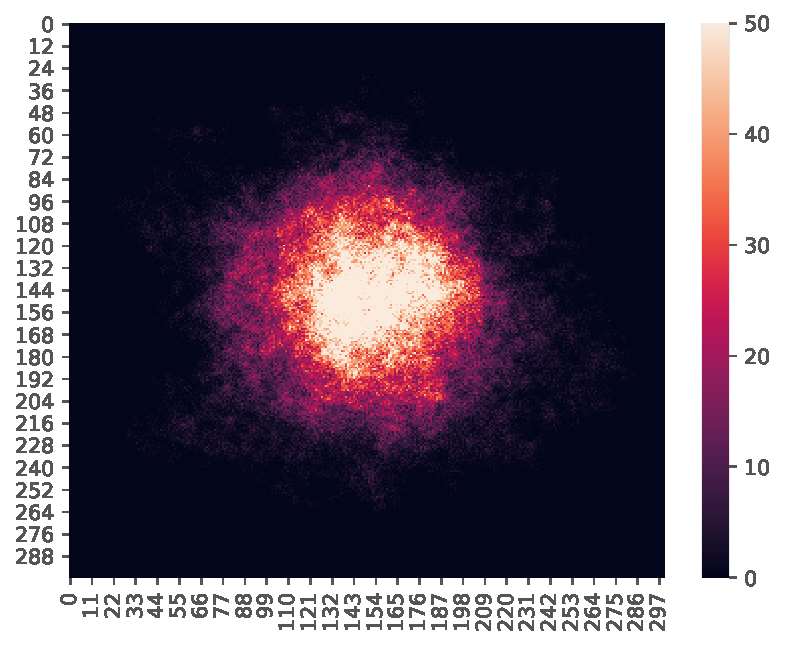
\includegraphics[trim=0cm 0.0cm 0cm 0cm,scale = 0.6]{D2_P_1I_N_Metropolis_S_2pow19_eqS_2pow18_Position_sampling_P_1_NH_2_I_0.pdf}
\caption{1 electron, $\hat E = 1$(a.u.)}
\label{J1}
\end{subfigure}
\begin{subfigure}[t]{.5\textwidth}
\centering
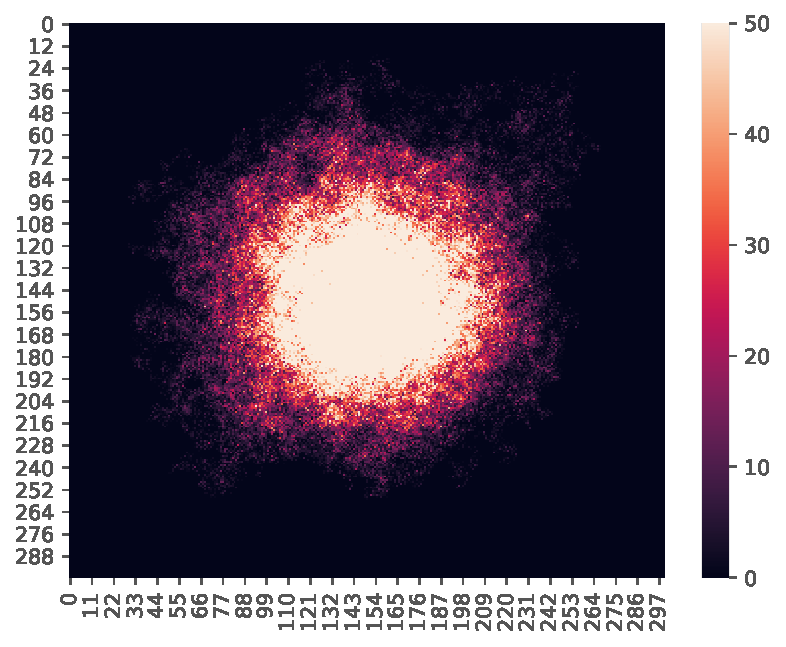
\includegraphics[trim=0cm 0.0cm 0cm 0.0cm,scale = 0.6]{D2_P_2I_N_Metropolis_S_2pow19_eqS_2pow18_Position_sampling_P_2_NH_2_I_0.pdf}
\caption{2 electrons, $\hat E = 2$(a.u.)}
\label{J2}
\end{subfigure}
\begin{subfigure}[b]{.5\textwidth}
\centering
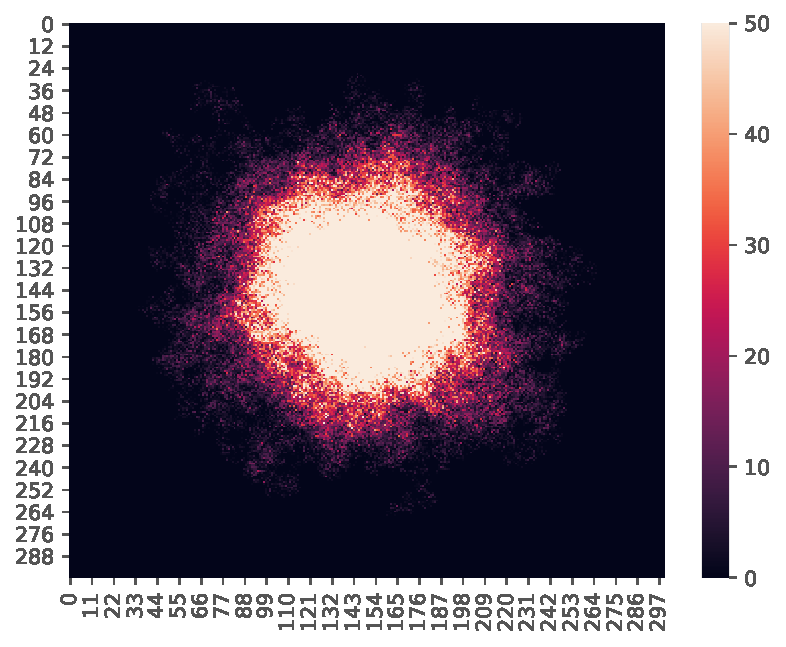
\includegraphics[trim=0cm 0.0cm 0cm 0.0cm,scale = 0.6]{D2_P_2I_Y_Metropolis_S_2pow19_eqS_2pow18_Position_sampling_P_2_NH_2_I_1.pdf}
\caption{2 interacting electrons, $\hat E = 3.29$(a.u.)}
\label{J1}
\end{subfigure}
\caption[as]{Electrons in two dimensions. Computed using importance sampling with $2^{18}$ equilibration steps, $2^{19}$ sampling steps and 200 learning steps. The entire interval in the x and y positions are six times the natural length scale of the system, centered at $x,y =0$. Those intervals are split into 300 zones that record each time an electron is located in that zone in the course of the sampling steps. }
\label{fig:Metropolis_pos_sampling}
\end{figure}


\subsubsection{Importance Sampling}
\begin{figure}[H]
\begin{subfigure}[t]{.5\textwidth}
\centering
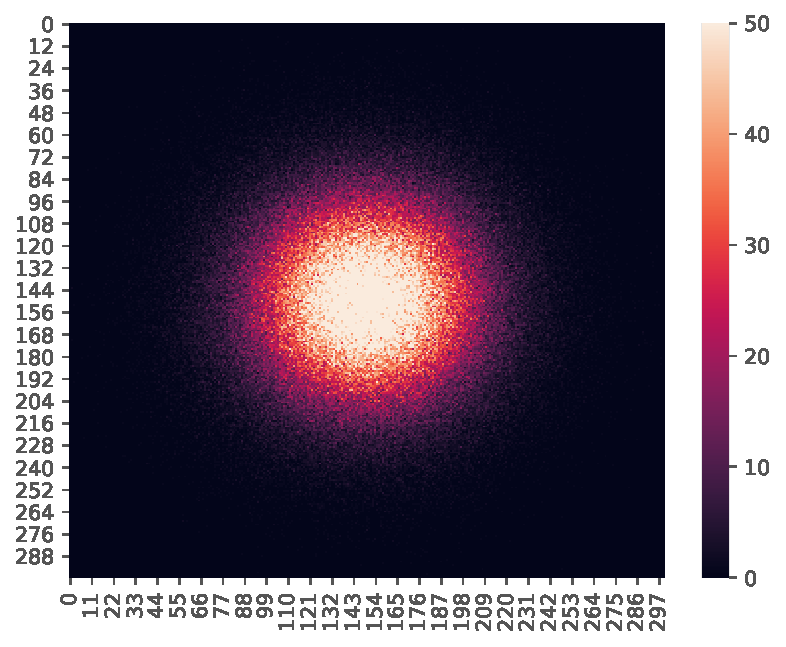
\includegraphics[trim=0cm 0.0cm 0cm 0cm,scale = 0.6]{D2_P_1I_N_Importance_S_2pow19_eqS_2pow18_Position_sampling_P_1_NH_2_I_0.pdf}
\caption{1 electron, $\hat E = 1$(a.u.)}
\label{imp1}
\end{subfigure}
\begin{subfigure}[t]{.5\textwidth}
\centering
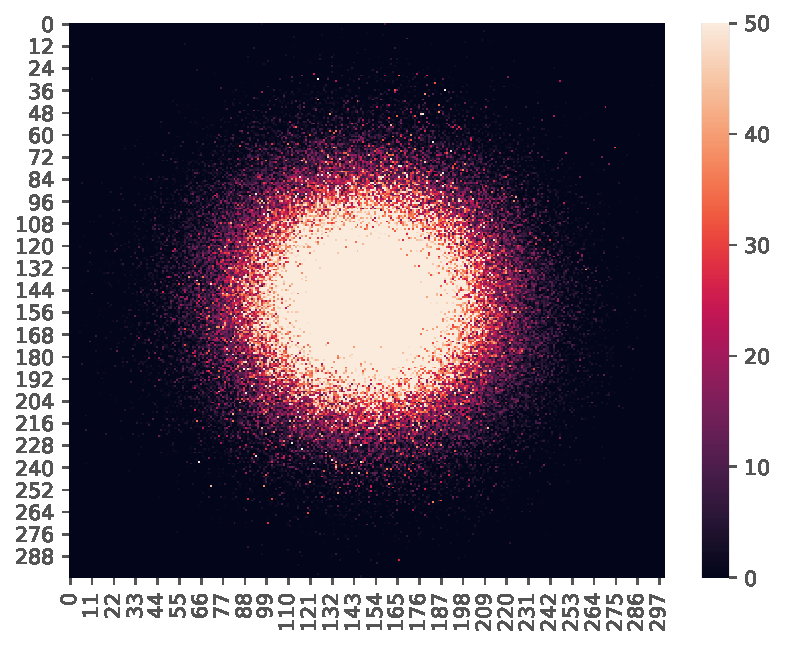
\includegraphics[trim=0cm 0.0cm 0cm 0.0cm,scale = 0.6]{D2_P_2I_N_Importance_S_2pow19_eqS_2pow18_Position_sampling_P_2_NH_2_I_0.pdf}
\caption{2 electrons, $\hat E = 2$(a.u.)}
\label{imp2}
\end{subfigure}
\begin{subfigure}[b]{.5\textwidth}
\centering
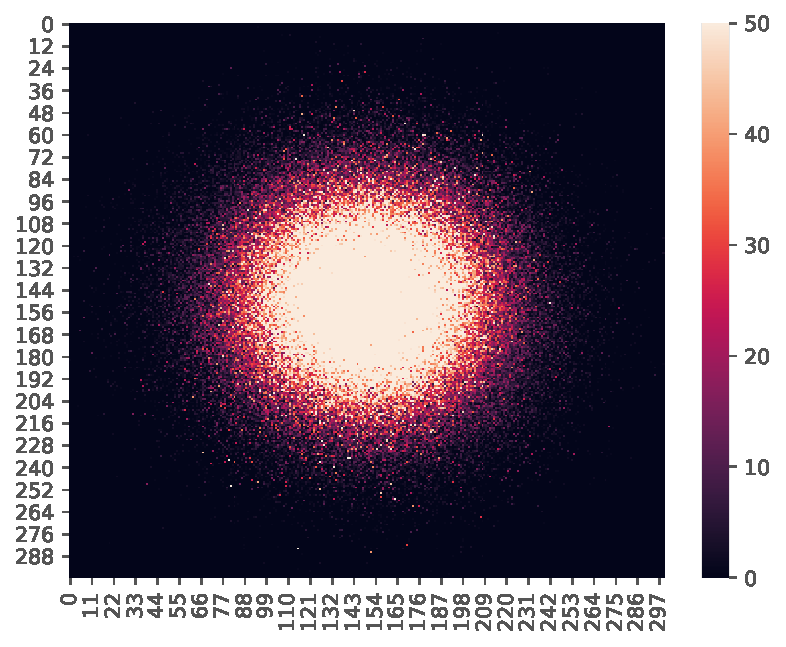
\includegraphics[trim=0cm 0.0cm 0cm 0.0cm,scale = 0.6]{D2_P_2I_Y_Importance_S_2pow19_eqS_2pow18_Position_sampling_P_2_NH_2_I_1.pdf}
\caption{2 interacting electrons, $\hat E = 3.24$(a.u.)}
\label{imp3}
\end{subfigure}
\caption[as]{Electrons in two dimensions. Computed using importance sampling with $2^{18}$ equilibration steps, $2^{19}$ sampling steps and 200 learning steps. The entire interval in the x and y positions are six times the natural length scale of the system, centered at $x,y =0$. Those intervals are split into 300 zones that record each time an electron is located in that zone in the course of the sampling steps. }
\label{fig:IMportance_pos_sampling}
\end{figure}
The vertical line is notably absent in figure \ref{imp1}, indicating that the faulty code does not lie with the interaction term, but with another function using the particles' x- position as an argument.
\subsection{Numerical instability}
A bug in an earlier implementation of this program would sometimes cause the energy of the system to explode. Now, I wouldn't normally include details about a bug, except that this one was quite interesting. Because of an indexing error, the y- coordinate of the second particle would never be updated in a metropolis step. The same indexing error also meant that if the move was rejected, the program would do something like this

\begin{algorithm}[H]
\SetAlgoLined
set $P_1(y) = P_2(x)$\;
set $P_2(x) = P_2(y) = Constant$\;
\end{algorithm}
effectively constraining the second particle to move along a small vertical line.
This meant that every time two moves were rejected in a row, we would get

\begin{algorithm}[H]
\SetAlgoLined
\KwResult{$P_1(y) = P_2(x) = P_2(y) = Constant$}
set $P_1(y) = P_2(x)$\;
set $P_2(x) = P_2(y)$\;
set $P_1(y) = P_2(x)$\;
set $P_2(x) = P_2(y)$\;
\end{algorithm}
This would (less strictly) constrain the first particle to align with the second, horizontally. The only (actual) degree of freedom for the system then became the x- position of the first particle. This created an obvious failure mode where every time the first particle crossed a diagonal ($P_1(x) = P_1(y)$), the interaction term would explode. The chance then, that the only relevant parameter ($P_1(x)$) would be updated in the next cycle was less than 1 in 3. The energy would then aggregate over several cycles and likely cause a memory leak. This problem would become worse, the closer the initial value of $P_2(y)$ was to zero, as the first particle would intercept the diagonal more frequently near the origin.\\One example of this failure mode is seen in figure \ref{fig:posSampling_unstable} below. The diagonal is marked in red. The x- and y- axes are flipped.
\begin{figure}[H]
\center
\begin{tikzpicture}
\node[inner sep=0pt] (russell) at (0,0)
    {\includegraphics[trim=0cm 0.3cm 0cm 0.0cm,scale = 0.6]{D2_P_2I_Y_Importance_S_2pow19_eqS_2pow18_Position_sampling_P_2_NH_2_I_1_Ene_ne1374.pdf}
};
\draw[red, thick, opacity = 0.1] (-3.4,3.0) -- (2.8,-2.7);
\end{tikzpicture}
\caption[numerically unstable run- electron positions]{Position sampling for 2 interacting electrons in 2 dimensions using importance sampling. In this case, the energy was calculated to be $-1374\hspace{1mm} a.u.$ The electrons remained at those locations for every sampling step. The second particle (most likely) is located on a diagonal, and the first (...) is horizontally locked to it.}
\label{fig:posSampling_unstable}
\end{figure}



\begin{figure}[H]
\center
\includegraphics[trim=0cm 0.3cm 0cm 0.0cm,scale = 0.6]{D2_P_2I_Y__S_2pow19_eqS_2pow18_GD_ls_v_E_LR_0.050000_NH_2.pdf}
\caption[numerically unstable run- electron positions]{2 interacting particles in 2 dimensions. Local energy as a function of SGD learning step using a learning rate of $0.05$. Sparse adverse events (large errorbars) stop SGD from converging properly}

\end{figure}
\section{Conclusion}


\section{Appendix A}\label{app_A}
Using the hamiltonian in \eqref{eq:hamiltonian} we get that the local energy is given by
$$
\begin{aligned}
E_{L} &=\frac{1}{\Psi} \mathbf{H} \Psi \\
&=-\frac{1}{2} \frac{1}{\Psi} \sum_{i}^{M} \frac{\partial^2}{\partial X_i^2} \Psi+\frac{1}{2} \omega^{2} \sum_{i}^{M} X_{i}^{2}+\sum_{j<k} \frac{1}{r_{j k}}
\end{aligned}
$$
with $M$ being the number of visible nodes in the network. The only non- trivial contribution comes from the Laplacian. We can simplify the differential term like this
$$
\frac{\partial^2}{\partial X_i^2} ln\Psi = \frac{\partial}{\partial X_i}\left( \frac{1}{\Psi}\frac{\partial}{\partial X_i} \Psi \right) = \frac{1}{\Psi}\frac{\partial^2}{\partial X_i^2} \Psi - \left( \frac{\partial}{\partial X_i} ln\Psi \right)^2
$$
giving us this expression

\begin{equation}\label{eq:local_energy_derived}
\begin{aligned}
E_{L} &=\frac{1}{\Psi} \mathbf{H} \Psi \\
&=-\frac{1}{2} \sum_{i}^{M} \left( \frac{\partial^2}{\partial X_i^2} ln\Psi +  \left( \frac{\partial}{\partial X_i} ln\Psi \right)^2 \right)+\frac{1}{2} \omega^{2} \sum_{i}^{M} X_{i}^{2}+\sum_{j<k} \frac{1}{r_{j k}}.
\end{aligned}
\end{equation}
Thankfully, the natural log of the wave function is easily computed to be
$$
ln\Psi = -ln Z-\sum_{i}^{M} \frac{\left(X_{i}-a_{i}\right)^{2}}{2 \sigma^{2}}+\sum_{j}^{N} ln \left(1+e^{b_{j}+\sum_{i}^{M} \frac{X_{i} W_{i j}}{\sigma^{2}}}\right).
$$
The differentials then become trivial to solve, and we get
$$
\frac{\partial}{\partial X_i} ln \Psi=\frac{1}{\sigma^{2}}\left(a_i-X_i+\sum_{j}^{N} W_{ij}\zeta(u_j) \right)
$$
and
$$
\frac{\partial^{2}}{\partial X_{i}^{2}} ln \Psi=-\frac{1}{\sigma^{2}}+\frac{1}{\sigma^{4}} \sum_{j}^{N} W_{i j}^{2} \zeta(u_j) \zeta(-u_j) 
$$
where $\zeta_j = \frac{1}{e^{-u_j}+1}$ is the familiar sigmoid function with $u_j = b_{j}+\frac{1}{\sigma^{2}} \sum_{k}^{M} X_k W_{k j}$. This concludes the calculation.
\section{Appendix B}\label{app_B}
The gradient of the local energy with respect to the network parameters is given by
\begin{equation}\label{eq:lE_gradient}
G_{i}=\frac{\partial\left\langle E_{L}\right\rangle}{\partial \alpha_{i}}=2\left(\left\langle E_{L} \frac{1}{\Psi} \frac{\partial \Psi}{\partial \alpha_{i}}\right\rangle-\left\langle E_{L}\right\rangle\left\langle\frac{1}{\Psi} \frac{\partial \Psi}{\partial \alpha_{i}}\right\rangle\right).
\end{equation}
From the expression for the wave function in \ref{app_A} the derivative of the wave function with respect to the weights and biases are easily calculated to be
$$
\frac{\partial}{\partial a_{i}} ln \Psi =\frac{X_{i}-a_{i}}{\sigma^{2}},
$$
$$
\frac{\partial}{\partial b_{i}} ln \Psi = \zeta_i
$$
and
$$
\frac{\partial}{\partial W_{i j}} ln \Psi =\frac{X_{i}}{\sigma^{2}}\zeta_j.
$$
this concludes the calculation.
\bibliographystyle{plain}
\bibliography{references}
\end{document}
